\section{Classified Image Based Performance Evaluation}

\subsection{Image-based VTON}

In this Section, we started with evaluating the 2D image based VTON algorithms. We considered CP-VTON\cite{Wang2018TowardCI} published in 2018 as the benchmark algorithm. The previous and following in 2019 share same input image and information conditions with CP-VTON and compare the results with it. Here we include the SCM based-VTON, VITON\cite{Han2017VITONAI}, and  CP-VTON\cite{Wang2018TowardCI}, however, we believe the performance strength and weakness are similar in the other algorithms too.


The Image based VTON algorithms are mostly composed of two stages: (1) cloth warping step that warps the try-on cloth to align with the pose and shape of the target model (called GMM in CP-VTON: geometric Manipulation Module)\cite{Wang2018TowardCI}, and (2) blending step that blends the warped cloth onto the target human image (called TON in CP-VTON: Try-On Network)\cite{Wang2018TowardCI}. CP-VTON assumes the target human image is pre-processed for a cloth agnostic human representation by a human pose estimation like OpenPose\cite{Cao2018OpenPoseRM} and human parsing like LIP\cite{Liang2018LookIP}. The human representation is composed of 1) heat maps for each joints 2) silhouette of human body, and 3) face and skin pixels patches (non-cloth and human identity area). We use the same dataset collected by Han et al. used in VITON\cite{Han2017VITONAI} and CP-VTON\cite{Wang2018TowardCI} papers.
 

\subsection{Classified quality}

Even though the success and failure cases are presented and compared with other algorithms' results, the failure case analysis is not enough for understanding the origin of failure cases and therefore difficult to find the solution for them. A classified evaluation would be better for this understanding. Here we summarized the classified results from our another study. We classify input try-on cloth and target human images according to the posture and body type of the person, the degree of occlusion of the clothes, and the characteristics of the clothes. Quality is compared in IoU for the warping step and in SSIM for the final blending step for same cloth re-try-on cases. We also tested for the new cloth try-on cases but did not include here for limitation of spaces, and the same cloth cases are enough to explain the tendencies of the performances. Though in general CP-VTON generates the best quality image, the relative comparison is not the main purpose of the analysis. Please refer to Figure \ref{fig:classified2DVTONresult} for detailed results.


\begin{figure}
\centering
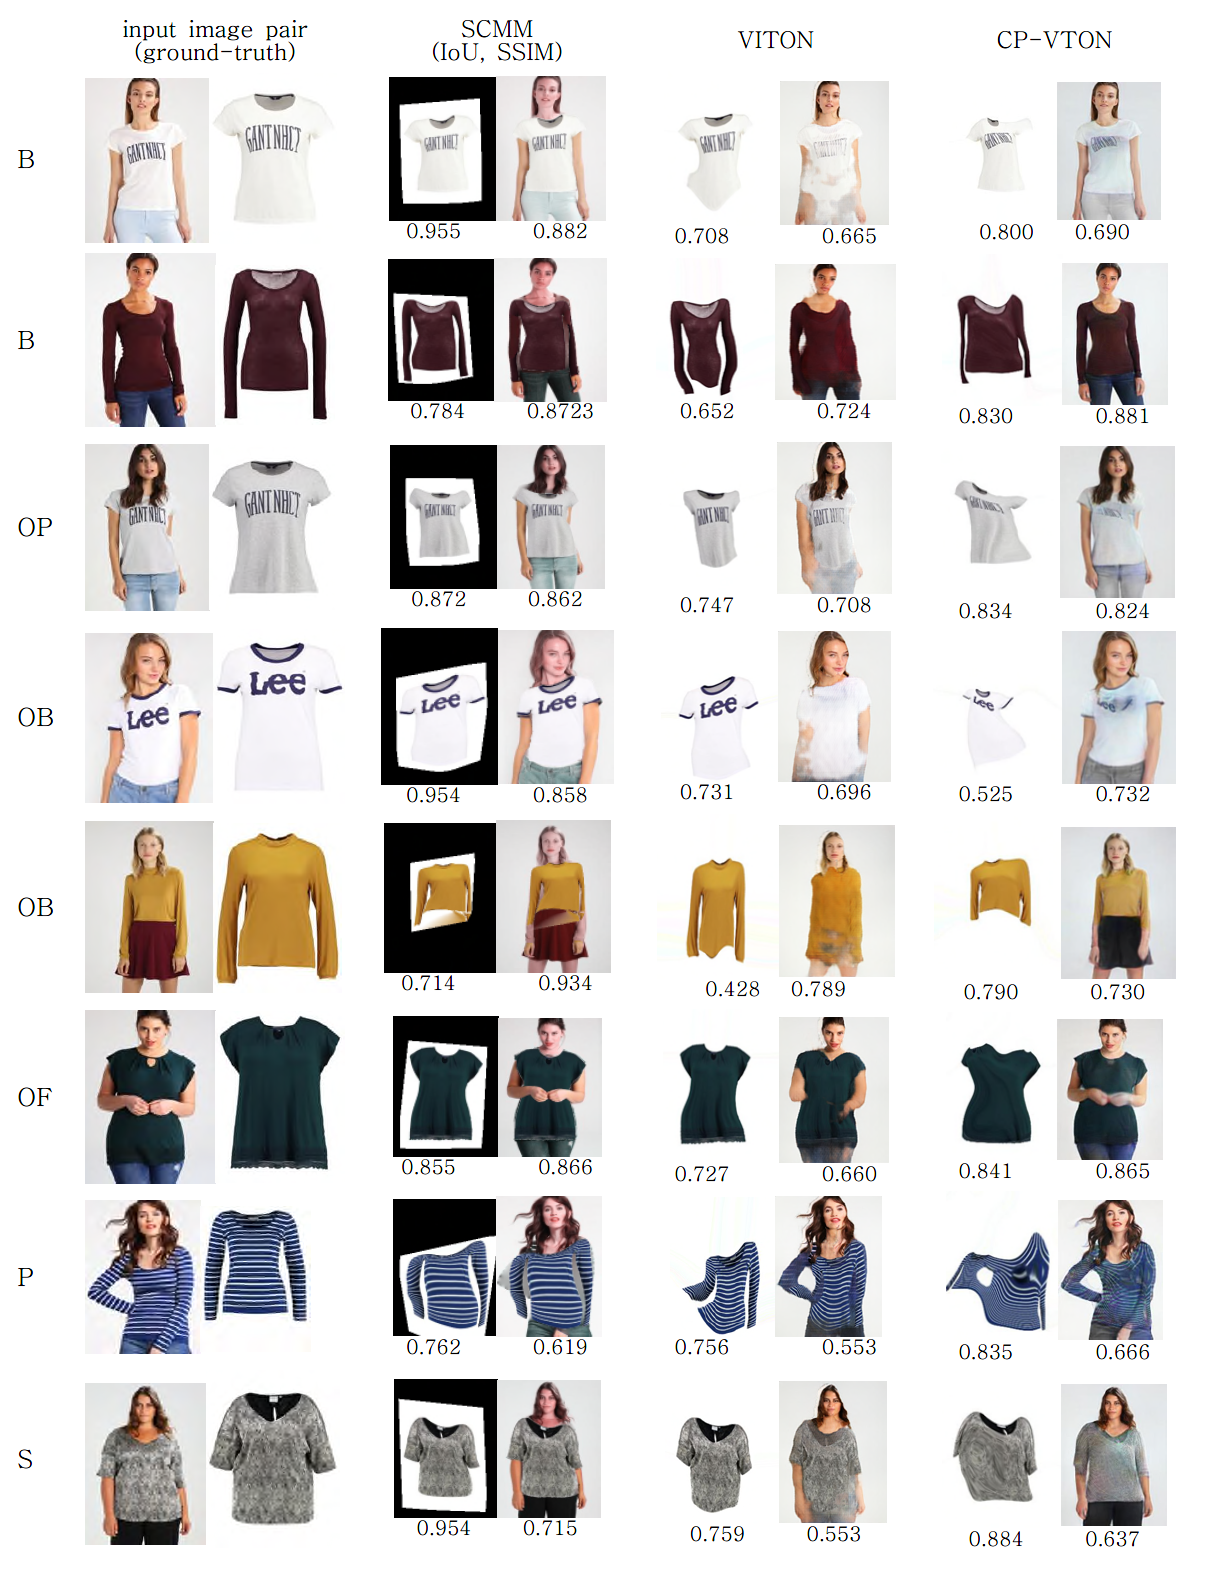
\includegraphics[height=13.5cm, scale=1]{figures/2dvton_same.png}   % TODO
\caption{Classified VTON result: same clothes}
\label{fig:classified2DVTONresult}
\end{figure}



////

Here I will describe the evaluation discussion, finally commenting that the GMM has serious problem.

////

Especially note that the warped cloth are often too much different for desired shape. It is originated two facts. First the 3D deformation that any 2D deformation including non-rigid transform such as TPS is quite limited, especially any 2D deformation cannot handle when the two area in the original image are overlapped in the destination images. There for when the arms of long sleeved cloth occlude the main body, 2D warping cannot approximate the 3D deformation properly. Second, the deformation needs corresponding points  between the source nd target image. The cloth are extremely difficult object to find the corresponding points. The STN (spatial transform network)\cite{JaderbergSZK15} and SCM (shape context matching)\cite{BelongieMP02} cannot find the corresponding points when the target cloth and original cloth has different shapes. In conclusion, the 2D image based algorithm has serious limitation in the range of applications. It can apply to the mild posed target human only and simple short sleeved cloth, mainly because the inherent limitation of 2D deformation method including non-rigid ones, and the poor performance of matching algorithm.  To overcome this limitation, we consider to model the try-on cloth into 3D model and apply the 3D deformation


